% Studentds question collection
%# Author Alejandro Gonzalez Recuenco and SKR students
%# e-mail <alejandrogonzalezrecuenco@gmail.com>

\documentclass{exam}
%SET-UP:
\usepackage{amsmath, physics, tikz, tcolorbox, graphicx}


%! TexExamRandomizer = {"noutput":2, "nquestions": [2,3,3,3,1,1]}
%! TexExamRandomizer = {"randominfo": {"randomnumber":100, "switchnumber":["even", "odd"]}}

\newcommand\myversion{0}
\newcommand\rseed{seed}



% DOCUMENT STARTS HERE
\begin{document}

\author{You version, \myversion}
\title{\textsc{Exam collection} --- mini-exam}


\maketitle


\begin{questions}

\section{Word problems}

	\question What is the mathematical definition of derivative.

	\begin{choices}
		\choice $f'(x) = \lim_{h\to 0}$ $\frac{f(x)-f(x)}{h+x}$
		\choice $f'(x) = \lim_{h\to 0}$ $\frac{f(x)-f(h)}{x}$
		\choice $f'(x) = \lim_{h\to 0}$ $\frac{f(x+h)+f(h)}{x}$
		\CorrectChoice $f'(x) = \lim_{h\to 0}$ $\frac{f(x+h)-f(x)}{h}$
	\end{choices}
	\question What is the derivative of the function $h(x) = \frac{f(x)}{g(x)}$,

	\begin{choices}
		\choice $h'(x) = f'(g(x)) \cdot g'(x).$
		\choice $h'(x) = f'(x)g(x)-f(x)g'(x).$
		\choice $h'(x) = f'(x)g(x)+f(x)g'(x).$
		\CorrectChoice $h'(x) = \frac{f(x)g'(x)-f'(x)g(x)}{(g(x))^2}.$
	\end{choices}

	\question Which one is the correct form of the chain rule ?

	\begin{choices}
		\choice $(f(g'))(x)=f'(g(x'))g'(x)$
		\choice $(f(g'))'(x)=f'(g(x'))g'(x)$
		\choice $(f(g))'(x)=f'(g'(x'))g'(x')$
		\CorrectChoice $(f(g))'(x)=f'(g(x))g'(x)$
	\end{choices}

	\question Which of the following is NOT a type of discontinuity?

	\begin{choices}
		\choice Removable.
		\choice Infinite jump.
		\choice Finite jump.
		\CorrectChoice Endpoint.
	\end{choices}

	\question What does a `Derivative' describe?
	\begin{choices}
		\choice It describes the instantaneous change of rate of the functions at $x$ axis.
		\choice It describes the instantaneous change of rate of the functions at $y$ axis.
		\choice It describes the instantaneous change of rate of the functions at some point.
		\CorrectChoice It describes the instantaneous change of rate of the functions at every point.
	\end{choices}
	\question What is a tangent line to a curve at a point $x = a$?

	\begin{choices}
		\choice A line that crosses a  curve once.
		\choice None of the other choices are correct.
		\choice A line that crosses a curve in two points.
		\CorrectChoice A line that has the same slope as the curve at the point $x = a$.
	\end{choices}
	\question What type of graph is the derivative of $f(x)= 5x^3+6x^2+5x-1$ graph?

	\begin{choices}
		\choice Line.
		\choice Circle.
		\choice Hyperbola.
		\CorrectChoice Parabola.
	\end{choices}
	\question The derivative of a function at a point $x = a$ tells us \ldots

	\begin{choices}
		\choice The limit of the function
		\choice The integral of the function.
		\choice The average rate of change.
		\CorrectChoice The slope of a tangent line of the graph at $x = a$.
	\end{choices}

\end{questions}

\begin{questions}

\section{Easy}
	\question If $y=\cos5x$ find $\dv{y}{x}$.

	\begin{choices}
		\choice $\dv{y}{x} = 5\cos5x$.
		\choice $\dv{y}{x} = -2\sin5x$.
		\choice $\dv{y}{x} = 5\cos2x$.
		\CorrectChoice $\dv{y}{x} = -5\sin5x$.
	\end{choices}
	\question Given $y=2x^2-3x+5$, What is $\dv[2]{y}{x}$

	\begin{choices}
		\choice $\dv[2]{y}{x}=4x-3$
		\choice $\dv[2]{y}{x}=16x-12$
		\choice $\dv[2]{y}{x}=0$
		\CorrectChoice $\dv[2]{y}{x}=4$
	\end{choices}
	\question What is the derivative of $y=\sin (2x + 5)$

	\begin{choices}
		\choice $ \cos(2x+5)$
		\CorrectChoice $ 2\cos(2x+5)$
		\choice $ 2\cos(2x)+5$
		\choice $ -2\cos(2x-5)$
	\end{choices}


	\question If the functions $f(x)$ and $g(x)$ are continuous everywhere then, what can we say about the function $h(x) = \frac{f(x)}{g(x)}$:

	\begin{choices}
		\CorrectChoice $\frac{f(x)}{g(x)}$ is also continuous everywhere except at the zeros of $g(x)$.
		\choice $h(x) = \frac{f(x)}{g(x)}$ is also continuous everywhere.
		\choice $h(x)$ will never cross the x axis.
		\choice More information is needed to answer this question.
	\end{choices}


	\question Find the value of $\lim_{x\to 2}\frac{x-1}{x^2-x-1}$

	\begin{choices}
		\choice $0$.
		\CorrectChoice $1$.
		\choice $\infty$.
		\choice Not possible.
	\end{choices}

	\question What is the derivative of $f(x)= 3x^4+2x^3-3x-2$
	\begin{choices}
		\choice $f'(x)= 3x^7+2x^6-3x^3-2$.
		\choice $f'(x)= 12x^3+6x^2-5$.
		\choice $f'(x)= 7x^4+5x^3-4x-2$.
		\CorrectChoice $f'(x)= 12x^3+6x^2-3$.
	\end{choices}
	\question What is the derivative of $(x^{2} + 3)(5 x + 2)$ ?

	\begin{choices}
		\choice $15 x^{2} + 19 x$
		\choice $50 x^{2} + 60 x$
		\choice $2 x + 5$
		\CorrectChoice $15 x^{2} + 4 x + 15$
	\end{choices}
	\question When $f'(x) = 0$ what happens?

	\begin{choices}
		\choice $f''(x) = 1$
		\choice $f''(x) = 0 $
		\CorrectChoice The point is a critical  point
		\choice Local maximum or minimum or an inflection point.
	\end{choices}
	\question What is the derivative of $f(x) = (2x+8)^2$

	\begin{choices}
		\choice $32$
		\choice $3x+32$
		\choice $4x+32$
		\CorrectChoice $8x+32$
	\end{choices}

	\question If $f(x) =\sqrt{x^3 - 4x}$, calculate when $f(x)=0 $

	\begin{choices}
		\choice $x = 0,\,1,\,{-1}$
		\choice $x= 0, $
		\choice $x= 0,\,2 $
		\CorrectChoice$ x= 0,\,2,\,{-2} $
	\end{choices}
	\question Given $f(x) = \frac{x^3-4}{2x+2}$, then $\lim_{x\to 4} f(x) = \ldots$

	\begin{choices}
		\choice $\ldots3.$
		\choice $\ldots4.$
		\choice $\ldots5.$
		\CorrectChoice $\ldots6.$
	\end{choices}
	\question  Suppose $f(x) = x^2 + 3$  and $g(x) = x - 2$. Which of the following is  $(f-g)(x)$?

	\begin{choices}
		\choice  $(f-g)(x)=x^2 - x +1$
     	\choice  $(f-g)(x)=x^3 + 2x^2 + 3x -2$
		\choice  $(f-g)(x)=x^2 - 4x + 7$
		\CorrectChoice   $(f-g)(x)=x^2 - x + 5$
	\end{choices}

	\question Given the functions $f(x) = x^4+3$ and $g(x) = \sqrt{x}$, find the value of $(f\circ g)'(x)\ldots$

	\begin{choices}
		\choice $(f\circ g)'(x) = x$
		\CorrectChoice $(f\circ g)'(x) = 2x$
		\choice $(f\circ g)'(x) = 3x$
		\choice $(f\circ g)'(x) = 4x$
	\end{choices}
	\question Which one is the correct form of the product rule?

	\begin{choices}
		\choice $(f(x)\cdot g(x))' = f'(x)g'(x)+f'(x)g'(x)$
		\choice $(f(x)\cdot g(x))' = f'(x)g'(x)+f(x)g(x)$
		\choice $(f(x)\cdot g(x))' = f(x)g'(x)+f(x)g'(x)$
		\CorrectChoice $(f(x)\cdot g(x))' = f'(x)g(x) + f(x)g'(x)$
	\end{choices}

	\question What is the derivative of $f(x) = \sqrt{4x+5}$

	\begin{choices}
		\choice $2\sqrt{x+5}$.
		\choice $8$.
		\choice $\frac{\sqrt{4x+5}}{2}$.
		\CorrectChoice $\frac{2}{\sqrt{4x+5}}$.
	\end{choices}
	\question Calculate the derivative of $f(x) = 2x^2+3$

	\begin{choices}
		\CorrectChoice $f'(x) = 4x$
		\choice $f'(x) = 2x$
		\choice $f'(x) = 5x$
		\choice $f'(x) = 6x$
	\end{choices}
	\question Calculate the derivative  of $y=\sin(3x{^2}+1)$

	\begin{choices}
		\choice $\dv{y}{x} = \sin(3x{^2}+1)$
		\choice $\dv{y}{x} = \cos(3x{^2}+1)$
        \choice $\dv{y}{x} = 6x\sin(3x{^2}+1)$
		\CorrectChoice $\dv{y}{x} = 6x \cos(3x{^2}+1)$
	\end{choices}
	\question Find the derivative of $f(x) = \sqrt[6]{4x+4}$

	\begin{choices}
		\choice $f'(x) = 4 (4x+4)^{-1/3} $
		\choice $f'(x) = \frac{4x }{6 \sqrt[3]{4x+4}}$
		\choice $f'(x) = \frac{4 x + 4}{6 \sqrt[6]{(4x + 4)^{5}}} $
		\CorrectChoice $f'(x) = \frac{4}{6 \sqrt[6]{(4x + 4)^{5}}}$
	\end{choices}

\end{questions}




\begin{questions}

\section{Medium}
	\question What is the derivative of f(x)=$(1-6x^2)^4$
	\begin{choices}
		\choice $4(1-6x^2)^3$
		\choice $4x(1-6x^2)^3$
		\choice $48x(1-6x^2)^3$
		\CorrectChoice $-48x(1-6x^2)^3 y$
	\end{choices}

	\question Find the slope of the tangent line of the curve $y = \frac{1}{x}$ at the point $(3,\frac13)$

	\begin{choices}
		\choice $\frac{1}{3}$
		\choice $\frac{-1}{3}$
		\choice $\frac{1}{9}$
		\CorrectChoice $\frac{-1}{9}$
	\end{choices}

	\question Calculate the following limit: $\lim_{x \to -2} = \frac{x^3+8}{x+2}\ $

	\begin{choices}
		\choice $\infty$.
		\choice $4$.
		\choice $1$.
		\CorrectChoice $12$.
	\end{choices}
	\question  Is this function continuous or discontinuous? $f(x) = \frac{x+8}{x-4}$

	\begin{choices}
		\choice  Continuous.
		\choice Discontinuous, contains a removable discontinuities.
		\choice No other answer is correct.
		\CorrectChoice Discontinuous, contains a jump discontinuities.
	\end{choices}

	\question $\displaystyle \lim_{x\to 4}{x^{2} + 2 x - 4}$ ?

	\begin{choices}
		\choice 14
		\choice 16
		\choice 18
		\CorrectChoice 20
	\end{choices}

	\question What is the name of the functions $\frac1{\cos x}$ ?
	\begin{choices}
		\choice $\csc x$
		\choice $\cot x$
		\choice $\tan x$
		\CorrectChoice $\sec x$
	\end{choices}

	\question Find the value of $\displaystyle \lim_{x \to 6} \frac{x^2 -36}{x^3 -216}$

	\begin{choices}
		\choice $\frac{1}{6}$
		\CorrectChoice $\frac{1}{9}$
		\choice $\frac{1}{12}$
		\choice $\frac{1}{15}$
	\end{choices}
	\question What is the function $f$ whose derivative is $f'(x)=x^5 +30$

    \begin{choices}
		\choice $f(x) = 5x^4 +30x$
		\choice $f(x) = 5x^4$
		\choice $f(x) = x^6 +30x$
		\CorrectChoice $f(x) = \frac{x^6}{6} +30x$
	\end{choices}
	\question Find the derivative of $f(x) = \frac{x-1}{x+1}$

	\begin{choices}
		\choice $f'(x) = \frac{-2}{(x+1)^2}$
		\choice $f'(x) = \frac{2}{(x-1)^2}$
		\choice $f'(x) = \frac{-2}{(x-1)^2}$
		\CorrectChoice $f'(x) = \frac{2}{(x+1)^2}$
	\end{choices}

\end{questions}




\begin{questions}

\section{Hard}
	\question  Calculate $\lim_{x\to 1}\frac{\sin (2x^2-2)}{x^2-1}$. (Hint: L'H\^opital rule)

	\begin{choices}
		\choice   $1$
		\choice  $-1$
		\choice  The limit does not exist.
		\CorrectChoice  $2$
	\end{choices}
	\question What is the local minimum of $x^3-2x^2$ in the range where $-1<x<1$?

	\begin{choices}
		\choice  $x=0$
		\choice  $x=-1$
		\choice There is no local minimum in that range.
		\CorrectChoice  $x=\frac43$
	\end{choices}
	\question What is the derivative of $f(x) = 2x \sin x + 2 \cos x - x^{2}\cos x.$

	\begin{choices}
		\choice $f'(x) = x^{2} \sin x + 2 x \cos x -2\sin x$.
		\choice $f'(x) = x^{2}\cos x$.
		\choice $f'(x) = 2x\cos x$.
		\CorrectChoice $f'(x) = x^{2}\sin x$.
	\end{choices}

	\question What is value of the $\displaystyle \lim_{h \to 0} \frac{f(x+h) -f(x)}{h}$ tells about the function?

	\begin{choices}
		\choice\label{choice:der1} The Slope of the graph.
		\choice\label{choice:der2} The critical point of the function , when the value of the limit is 0.
		\CorrectChoice Both options, \ref{choice:der1} and \ref{choice:der2}, are correct.
		\choice None of the above.
	\end{choices}

	\question What is the derivative of $f(x) = \arctan(2x)$ ?

	\begin{choices}
		\choice $\frac{2}{1 + x^{2}}$
		\choice $\frac{2}{2 + x^{2}}$
		\choice $\frac{2}{2 + 4x^{2}}$
		\CorrectChoice $\frac{2}{1 + 4x^{2}}$
	\end{choices}
	\question Find the derivatives of f(x) = $\sin^6(x^4)$

	\begin{choices}
		\choice $6\sin^{5}(x^4)$
		\choice $24 x^{3}\sin(x^3) \sin(x^4)$
		\choice $24\sin(x^4)  \cos(x^3)$
		\CorrectChoice $24 x^{3} \sin^{5}(x^4)  \cos(x^4) $
	\end{choices}
	\question Find the derivative of $f(x)$ = $\sqrt{x^2+3x}$.

	\begin{choices}
		\choice $f'(x) = \frac{1}{2}\sqrt{2x+3}$.
		\choice $f'(x) = \frac{1}{x^2+3x}(2x+3)$.
		\choice $f'(x) = \frac{-1}{2 \sqrt{2x + 3}}$.
		\CorrectChoice $f'(x) = \frac{2x + 3}{2 \sqrt{2x + 3}}$.
	\end{choices}


\end{questions}


\begin{questions}
\section{Graphic problems}
	\question
	From the following graph find $\lim_{x \to -2 } f(x)$
	\par\nopagebreak
	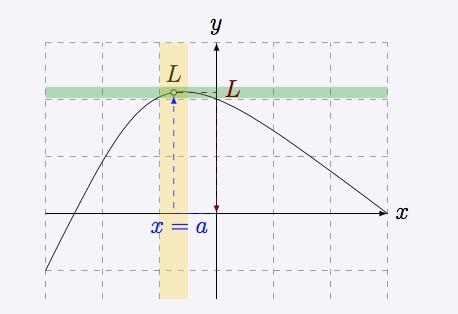
\includegraphics[width = 6cm]{limgraph.jpg}

	\begin{choices}
		\choice $0$.
		\choice $5$.
		\choice $4$.
		\CorrectChoice undefined.
	\end{choices}

\end{questions}


\begin{questions}
\section{Bonus, integration}
	\question Find the area of the graph between f(x) = $x^4$ and f(x) = $(x-6)^4$

	\begin{choices}
		\choice $\frac{243}{5}$
		\choice $\frac{243}{10}$
		\choice $\frac{486}{10}$
		\CorrectChoice $\frac{486}{5}$
	\end{choices}
	\question Find the integral of $ 4x^3+3x^2 $

	\begin{choices}
		\choice $12x^2 + 6x$
		\choice $4x^2 + 3x$
		\choice $4x^4 + 3x^3 + c$
		\CorrectChoice $x^4 + x^3 +c$
	\end{choices}
	\question What is the area under the graph $y = x^3$, the line $y = 0$ and the lines $x=0$ and $x=2$?

	\begin{choices}
		\choice 8
		\choice 16
		\choice 24
		\CorrectChoice 4
	\end{choices}
	\question Which of these processes are used to calculate the area under a curve?
	\begin{choices}
		\choice First derivative
		\choice Product rule
		\choice Second derivative
		\CorrectChoice Integral
	\end{choices}




\end{questions}

\end{document}
